%\documentclass[notitlepage,aps,prd,twocolumn,nofootinbib]{revtex4-1}
\documentclass[notitlepage,aps,prd,nofootinbib]{revtex4-1}

\usepackage{subfig}
%\usepackage[colorinlistoftodos]{todonotes}
\usepackage{float}

%\usepackage[protrusion=true,expansion=true]{microtype}
\usepackage{amsmath}
\usepackage{amssymb}
\usepackage{bbm}
\usepackage{ulem}
%\usepackage{feynmp-auto}
%\usepackage{slashed}
%\usepackage[absolute,overlay]{textpos}
\usepackage[usenames, dvipsnames]{color}
\usepackage{graphicx}
\usepackage{listings}
\usepackage{epsfig}
\usepackage{hyperref}
%\usepackage{tikz}
\usepackage{enumerate}
%\usepackage{fixltx2e} % buggy
\usepackage[compatibility=false]{caption}
%\usepackage{subcaption} % doesn't work with subfigure
\usepackage{pdfpages}
%\usepackage{setspace}
\usepackage{verbatim}

% Turn of meaningless float warnings
\usepackage{silence}
\WarningFilter{revtex4-1}{Repair the float}

\DeclareRobustCommand{\orderof}{\ensuremath{\mathcal{O}}}

\definecolor{dukeblue}{RGB}{0,0,156}
\definecolor{dukedarkblue}{RGB}{0,26,87}
\definecolor{dukeblack}{RGB}{79,79,79}
\definecolor{dukegray}{RGB}{79,79,79}
\definecolor{dukesecbrown}{RGB}{217,200,158}
\definecolor{dukesecblue}{RGB}{127,169,174}

%\renewcommand*{\thefootnote}{\fnsymbol{footnote}}

%%%%%%%%%%%%%%%%%%%%%%%%%%%%%%%%%%%%%%%%%%%%%%%%%%%%%%%%%%%%%%%%%%%%%%%%%%%%%%%%%%%%%
\hypersetup{
    breaklinks,
    baseurl       = http://,
    pdfborder     = 0 0 0,
    pdfpagemode   = UseNone,% do not show thumbnails or bookmarks on opening
    pdfstartpage  = 1,
    bookmarksopen = true,
    bookmarksdepth= 2,% to show sections and subsections
% revtex needs author and title declared after \begin{document}, so have to hard code them...
%    pdfauthor     = {\@author},
%    pdftitle      = {\@title},
    pdfauthor     = {Matthew Epland},
    pdftitle      = {Phys 566 HW3},
    pdfsubject    = {},
    pdfkeywords   = {}}


% Code import settings
%%%%%%%%%%%%%%%%%%%%%%%%%%%%%%%%%%%%%%%%%%%%%%%%%%%%%%%%%%%%%%%%%%%%%%%%%%%%%%%%%%%%%
\definecolor{mygreen}{rgb}{0,0.6,0}
\definecolor{mygray}{rgb}{0.5,0.5,0.5}
\definecolor{mymauve}{rgb}{0.58,0,0.82}

%\lstset{ %
\lstdefinestyle{python}{ %
  backgroundcolor=\color{white},   % choose the background color; you must add \usepackage{color} or \usepackage{xcolor}
  basicstyle=\scriptsize,          % the size of the fonts that are used for the code
  breakatwhitespace=false,         % sets if automatic breaks should only happen at whitespace
  breaklines=true,                 % sets automatic line breaking
  captionpos=b,                    % sets the caption-position to bottom
  commentstyle=\color{mygreen},    % comment style
  deletekeywords={...},            % if you want to delete keywords from the given language
  escapeinside={\%*}{*)},          % if you want to add LaTeX within your code
  extendedchars=true,              % lets you use non-ASCII characters; for 8-bits encodings only, does not work with UTF-8
  frame=single,	                   % adds a frame around the code
  keepspaces=true,                 % keeps spaces in text, useful for keeping indentation of code (possibly needs columns=flexible)
  keywordstyle=\color{blue},       % keyword style
  language=Python,                 % the language of the code
  otherkeywords={*,...},           % if you want to add more keywords to the set
  numbers=left,                    % where to put the line-numbers; possible values are (none, left, right)
  numbersep=5pt,                   % how far the line-numbers are from the code
  numberstyle=\tiny\color{mygray}, % the style that is used for the line-numbers
  rulecolor=\color{black},         % if not set, the frame-color may be changed on line-breaks within not-black text (e.g. comments (green here))
  showspaces=false,                % show spaces everywhere adding particular underscores; it overrides 'showstringspaces'
  showstringspaces=false,          % underline spaces within strings only
  showtabs=false,                  % show tabs within strings adding particular underscores
  stepnumber=5,                    % the step between two line-numbers. If it's 1, each line will be numbered
  stringstyle=\color{mymauve},     % string literal style
  tabsize=2,	                   % sets default tabsize to 2 spaces
%  title=\lstname                   % show the filename of files included with \lstinputlisting; also try caption instead of title
  title={\protect\filename@parse{\lstname}\protect\filename@base.\filename@ext},
  firstnumber=0,
%  linewidth=0.95\textwidth
  xleftmargin=0.01\textwidth,
  xrightmargin=0.01\textwidth
}

\lstdefinestyle{output}{ %
  backgroundcolor=\color{white},   % choose the background color; you must add \usepackage{color} or \usepackage{xcolor}
  basicstyle=\scriptsize,          % the size of the fonts that are used for the code
  breakatwhitespace=false,         % sets if automatic breaks should only happen at whitespace
  breaklines=true,                 % sets automatic line breaking
  captionpos=b,                    % sets the caption-position to bottom
  escapeinside={\%*}{*)},          % if you want to add LaTeX within your code
  frame=single,	                   % adds a frame around the code
  keepspaces=true,                 % keeps spaces in text, useful for keeping indentation of code (possibly needs columns=flexible)
  numbers=left,                    % where to put the line-numbers; possible values are (none, left, right)
  numbersep=5pt,                   % how far the line-numbers are from the code
  numberstyle=\tiny\color{mygray}, % the style that is used for the line-numbers
  rulecolor=\color{black},         % if not set, the frame-color may be changed on line-breaks within not-black text (e.g. comments (green here))
  stepnumber=5,                    % the step between two line-numbers. If it's 1, each line will be numbered
  tabsize=2,	                   % sets default tabsize to 2 spaces
%  title=\lstname                   % show the filename of files included with \lstinputlisting; also try caption instead of title
  title={\protect\filename@parse{\lstname}\protect\filename@base.\filename@ext},
  firstnumber=0,
%  linewidth=0.95\textwidth
  xleftmargin=0.01\textwidth,
  xrightmargin=0.01\textwidth
}

% Select between raw and saved plots here
\graphicspath{{../code/output/}} % raw plots
%\graphicspath{{./output/}} % saved plots

%%%%%%%%%%%%%%%%%%%%%%%%%%%%%%%%%%%%%%%%%%%%%%%%%%%%%%%%%%%%%%%%%%%%%%%%%%%%%%%%%%%%%
\begin{document}

\title{PHYS 566 HW3}
\author{Matthew Epland}
\affiliation{Department of Physics, Duke University, Durham, NC 27707, USA}
%\institute{Duke University}

\date{\today}

\begin{abstract}
TODO
\end{abstract}\maketitle


\section{Introduction}
\label{sec:intro}
TODO

\section{Theory}
\label{sec:theory}
We can numerically model an objects trajectory by splitting up Newton's 2nd Law (\ref{eq:newton2}) into coupled first order differential equations (\ref{eq:deqs}) that we can apply the Euler method (\ref{eq:r_euler} and \ref{eq:v_euler}) to.

\begin{equation} \label{eq:newton2}
m \frac{d^{2} \mathbf{r}}{d t^{2}} = \mathbf{F}_{\text{net}} 
\end{equation}

\begin{equation} \label{eq:deqs}
\frac{d \mathbf{v}}{d t} = \frac{1}{m} \mathbf{F}_{\text{net}}
\qquad
\frac{d \mathbf{r}}{d t} = \mathbf{v}
\end{equation}

\begin{equation} \label{eq:r_euler}
\mathbf{r}\left(t + \Delta t\right) \approx \mathbf{r}\left(t\right) + \frac{d \mathbf{r}}{d t} \Delta t = \mathbf{r}\left(t\right) + \mathbf{v}\left(t\right) \Delta t
\end{equation}

\begin{equation} \label{eq:v_euler}
\mathbf{v}\left(t + \Delta t\right) \approx \mathbf{v}\left(t\right) + \frac{d \mathbf{v}}{d t} \Delta t = \mathbf{v}\left(t\right) + \frac{1}{m}\mathbf{F}_{\text{net}}\left(t\right) \Delta t
\end{equation}

These equations are the heart of our model. All we need do now is split the vectors up into components, $\hat{\mathbf{x}}$ along the ground and $\hat{\mathbf{y}}$ vertical, by performing some simple trigonometry (\ref{eq:vartheta}) with $\vartheta$ defined as the angle from horizontal i.e.\ $\hat{\mathbf{x}}$, and set the initial conditions (\ref{eq:initial_conditions}).

\begin{equation} \label{eq:vartheta}
\vartheta\left(t\right) = \arctan\left(\frac{v_{y}(t)}{v_{x}(t)}\right)
\qquad
\mathbf{v}\left(t\right) = v\left(t\right)
\begin{pmatrix}
  \cos(\vartheta) \\
  \sin(\vartheta)
\end{pmatrix}
\end{equation}

\begin{equation} \label{eq:initial_conditions}
\mathbf{r}\left(0\right) = 
\begin{pmatrix}
  0 \\
  0
\end{pmatrix}
\qquad
\mathbf{v}\left(0\right) = v_{0}
\begin{pmatrix}
  \cos(\vartheta_{0}) \\
  \sin(\vartheta_{0})
\end{pmatrix}
\end{equation}


In this assignment we are considering gravity as well as drag forces in four different cases:

\subsection{Ideal Object} \label{subsec:ideal}
Without drag $\mathbf{F}_{\text{net}}$ (\ref{eq:F_ideal}) is very straight forward as only gravity acts on the object, and even then only along one axis.

\begin{equation} \label{eq:F_ideal}
\mathbf{F}_{\text{net}} = -m g~\hat{\mathbf{y}}
\end{equation}

\subsection{Smooth Object with Drag} \label{subsec:smooth_drag}
A simple approximation of the laminar flow drag force over a smooth surface is $\mathbf{F}_{\text{drag}} = - C \rho A v^{2}~\hat{\mathbf{v}}$, where $C = 1/2$, $\rho$ is the density of surrounding fluid, and $A$ is the frontal area of the object. Adding this form of drag to the ideal case results in (\ref{eq:F_smooth_drag}).

\begin{equation} \label{eq:F_smooth_drag}
\mathbf{F}_{\text{net}} = - \frac{1}{2} \rho A v^{2} 
\begin{pmatrix}
  \cos(\vartheta) \\
  \sin(\vartheta)
\end{pmatrix}
-m g~\hat{\mathbf{y}}
\end{equation}


\subsection{Dimpled Object with Drag} \label{subsec:dimpled_drag}
We can increase the complexity of the problem by allowing the object's surface to be dimpled, like a golf ball. $\mathbf{F}_{\text{drag}} = - C \rho A v^{2}~\hat{\mathbf{v}}$ will still work in this case, but now we let $C$ become a piecewise function of the object's speed (\ref{eq:Cv}). This is done to account for the switch between laminar flow at low speeds, where the dimples effects are negligible and $\mathbf{F}_{\text{drag}} \propto v^{2}$, and turbulent flow at high speeds, where the dimples break up the air flow over the object's surface and allow it to maintain contact longer. The air flow thus sticks close to the surface further along it's length, thereby reducing the overall wake vortex and drag, which is equivalent to letting $\mathbf{F}_{\text{drag}} \propto v$. With this modification our $\mathbf{F}_{\text{net}}$ equation becomes (\ref{eq:F_dimpled_drag}).

\begin{equation} \label{eq:Cv}
C\left(v\right) =
  \begin{cases} 
    \frac{1}{2} & v \leq v_{\text{transition}} \\
    \\
    \frac{C'}{v} & v \geq v_{\text{transition}}
  \end{cases}
\qquad \text{where} \qquad
C' \leq \frac{v_{\text{transition}}}{2}
\end{equation}

\begin{equation} \label{eq:F_dimpled_drag}
\mathbf{F}_{\text{net}} = - C\left(v\right) \rho A v^{2}
\begin{pmatrix}
  \cos(\vartheta) \\
  \sin(\vartheta)
\end{pmatrix}
-m g~\hat{\mathbf{y}}
\end{equation}

\subsection{Dimpled Object with Drag and Spin} \label{subsec:dimpled_drag_spin}
Lastly, we can allow the object to spin in addition to the drag force considered earlier. In particular we will be considering objects with back spin, like a golf ball after it leaves the club. The objects spin will make the relative velocity of the surrounding fluid over the object's surface a function of position, thereby creating uneven drag forces. We can model this effect with a Magnus force, $\mathbf{F}_{\text{Magnus}} = S_{0}~\vec{\omega} \times \mathbf{v}$. In our coordinate system backspin corresponds to having $\hat{\omega} = \hat{\mathbf{z}}$ out of the page. With this in mind we can perform the cross product, break $\mathbf{F}_{\text{Magnus}}$ into its components, and compute the new $\mathbf{F}_{\text{net}}$ (\ref{eq:F_dimpled_drag_and_spin}).

\begin{equation} \label{eq:F_dimpled_drag_and_spin}
\mathbf{F}_{\text{net}} = S_{0} \omega v 
\begin{pmatrix}
  \cos(\vartheta + \frac{\pi}{2}) \\
  \sin(\vartheta + \frac{\pi}{2})
\end{pmatrix}
- C\left(v\right) \rho A v^{2}
\begin{pmatrix}
  \cos(\vartheta) \\
  \sin(\vartheta)
\end{pmatrix}
-m g~\hat{\mathbf{y}}
\end{equation}

It is convenient to define one constant $\eta \equiv \frac{S_{0} \omega}{m}$ to hold the $S_{0}$ and $\omega$ dependence. Making this substitution and simplifying the trigonometry leaves us with the final form of $\mathbf{F}_{\text{net}}$ (\ref{eq:F_dimpled_drag_and_spin_2}). 

\begin{equation} \label{eq:F_dimpled_drag_and_spin_2}
\mathbf{F}_{\text{net}} = m \eta v 
\begin{pmatrix}
  -\sin(\vartheta) \\
  \cos(\vartheta)
\end{pmatrix}
- C\left(v\right) \rho A v^{2}
\begin{pmatrix}
  \cos(\vartheta) \\
  \sin(\vartheta)
\end{pmatrix}
-m g~\hat{\mathbf{y}}
\end{equation}


\section{Results}
\label{sec:results}
TODO

\begin{figure}[!htbc]
  \centering
  \includegraphics[width=.70\textwidth]{ideal.png}
	{\par\nobreak\rule[9pt]{35em}{0.5pt}\vspace{-5mm}}
	\caption{Trajectories of an ideal ball without drag at different initial elevations, $\vartheta_{0}$.}
	\label{fig:ideal}
\end{figure}



\begin{figure}[!htbc]
  \centering
  \includegraphics[width=.70\textwidth]{smooth_ball_w_drag.png}
	{\par\nobreak\rule[9pt]{35em}{0.5pt}\vspace{-5mm}}
	\caption{Trajectories of a smooth ball with drag at different initial elevations, $\vartheta_{0}$.}
	\label{fig:smooth_ball_w_drag}
\end{figure}

\begin{figure}[!htbc]
  \centering
  \includegraphics[width=.70\textwidth]{dimpled_ball_w_drag.png}
	{\par\nobreak\rule[9pt]{35em}{0.5pt}\vspace{-5mm}}
	\caption{Trajectories of a dimpled ball with drag at different initial elevations, $\vartheta_{0}$.}
	\label{fig:dimpled_ball_w_drag}
\end{figure}



\section{Conclusions}
\label{sec:Conclusions}
TODO

The Python source code used to produce these results can be found online at \url{http://github.com/mepland/PHYS_566_Computational_HW/tree/master/hw3/code}, and is included in Section~\ref{sec:code}.

\clearpage
\section{Supporting Material}
\label{sec:Supporting_Material}

% TODO output.log

\clearpage
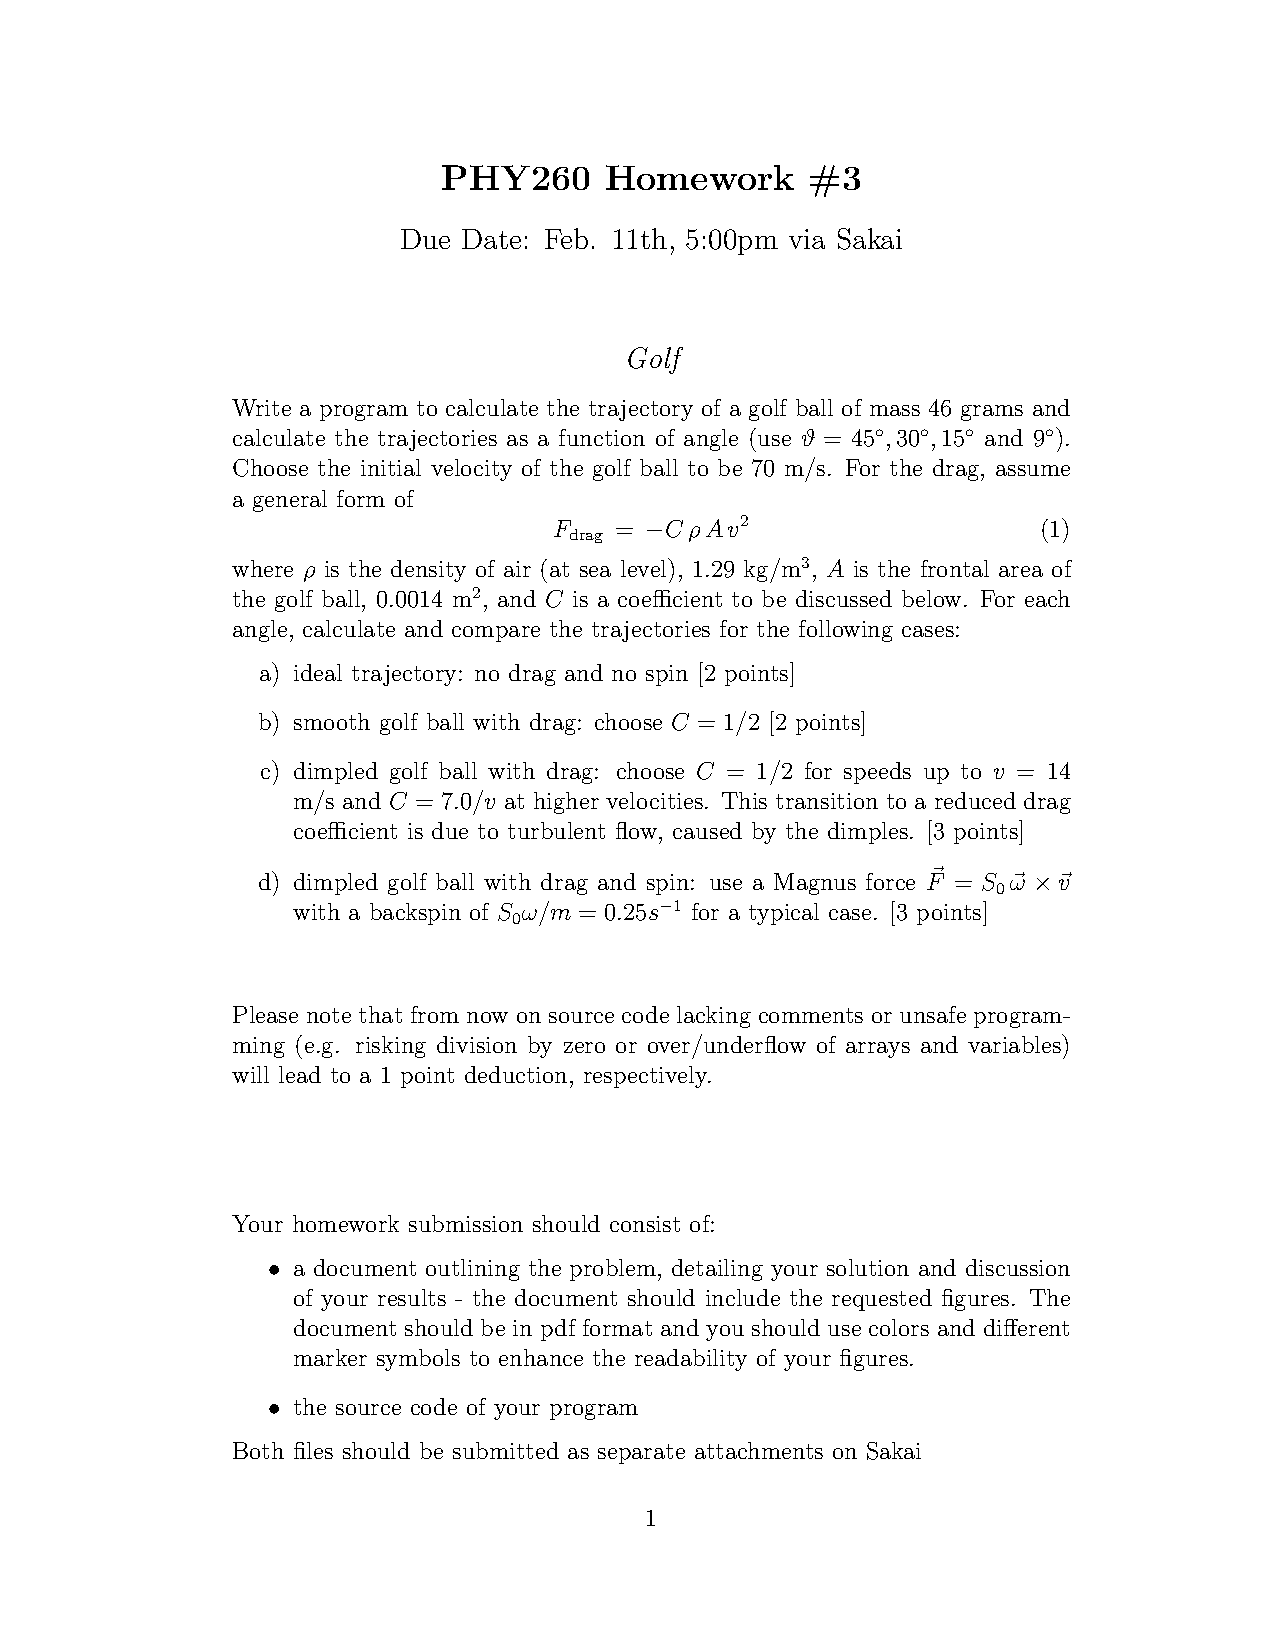
\includepdf{../homework3.pdf}

\clearpage
\section{Code}
\label{sec:code}

\lstinputlisting[style=python]{../code/golf.py}

\end{document} %%% end of doc %%%




\bibliographystyle{bib_files/styles/atlasBibStyleWoTitle}
\bibliography{bib_files/my_bib.bib}


